\documentclass[range]{ar2e}
       
\usepackage{amsmath}
\usepackage{color}
\usepackage{verbatim}
\usepackage{graphicx}
\usepackage{wasysym}
\usepackage{amssymb}

                           
\begin{document}

\input epsf.def
\input psfig.sty



%\jname{Annual Reviews of Condensed Matter Physics}
%\jyear{2012}
%\jvol{XX}
%\ARinfo{1056-8700/97/0610-00}

\title{Designer Hamiltonians---bridging lattice-scale physics \\ and continuum field theory with 
quantum Monte Carlo simulations} 

\author{Ribhu K. Kaul
\affiliation{Department of Physics and Astronomy, University of Kentucky, Lexington, Kentucky 40506, USA}
Roger G. Melko
\affiliation{Department of Physics and Astronomy, University of Waterloo, Ontario, N2L 3G1, Canada}
\affiliation{Perimeter Institute for Theoretical Physics, Waterloo, Ontario N2L 2Y5, Canada}
Anders W. Sandvik
\affiliation{Department of Physics, Boston University, 590 Commonwealth Avenue, Boston, Massachusetts 02215, USA}}

\begin{abstract}
We discuss designer Hamiltonians---lattice models tailored to be free from sign problems when simulated with quantum 
Monte Carlo methods but still host complex  many-body states and quantum phase transitions of great interest in condensed matter 
physics. We here focus on quantum spin systems in which competing interactions lead to non-magnetic ground states. These states and 
associated quantum phase transitions can be studied in great detail, enabling direct access to universal properties and connections 
with low-energy effective quantum field theories. As specific examples, we discuss the transition from a N\'eel antiferromagnet to 
either a uniform quantum paramagnet or a spontaneously symmetry-broken valence-bond-solid in SU($2$) and SU($N$) spin models. We also 
discuss anisotropic (XXZ) systems harboring spin liquids and the XY$^*$ transition. We briefly review recent progress on quantum Monte 
Carlo algorithms, including ground state projection in the valence-bond basis and direct computation of the Renyi variants of the 
entanglement entropy.
\end{abstract}

\maketitle

\section{Introduction}
\label{sec:intro}

Quantum field theory has emerged as one of the most fruitful approaches for studying low-energy properties of
complex strongly correlated and entangled quantum matter systems. There are potential pitfalls and difficulties 
with this approach, however, and it is, therefore, important to also study systems directly based on the Hamiltonian 
formulation. One of the most fruitful directions here is to use numerical methods to study lattice Hamiltonians 
in an unbiased way, and to extract from such calculations the relevant low-energy emergent properties that can 
be compared with results for corresponding quantum field theories. Such connections between the two approaches 
can have significant synergy effects in advancing our understanding of many-body phenomena. Computational studies 
have their own challenges, however, and most systems of interest are currently beyond the reach of existing 
numerical algorithms. Frustrated quantum spin systems and fermions in two and three dimensions are the two main 
groups of problematic systems. The approach we review here is to tailor particular ``designer hamiltonians'', which 
can host ground states and quantum phase transitions of interest and also are amenable to large-scale numerical 
studies. The main computational technique we have in mind is quantum Monte Carlo (QMC) simulation, which in the 
aforementioned systems are normally affected by the infamous ``sign problem'',\cite{Loh90,Henelius00} i.e., the 
weight function in the configuration space constructed using the path integral or other mappings to an effective 
statistical-mechanics problem is not positive definite (and hence cannot be directly used as a probability 
distribution for importance sampling).

A common misunderstanding is that interesting designer Hamiltonians should not exist---if a model is sign-problem 
free it will likely be trivial or uninteresting. There are already many counter-examples to this pessimistic view, however, 
and we will here review some recent examples from the area of quantum magnetism. Recent advances in QMC methods have made 
it possible to truly approach the low-energy limit of many models and to make detailed connections with field theories. 
We will brifly address some of these technical advances as well. First, further remark on field theory and the philosophy 
of the synergistic use of designer hamiltonians.

\subsection{Field theory and numerical studies of Hamiltonians}

A field theory can rarely be rigorously derived exactly from 
an underlying Hamiltonian (which is the natural starting point for describing condensed matter systems). Instead
it is constructed based on symmetries, in combination with insights or assumptions on the physical nature of the
system. Some times the field theory can be derived in some well defined limit, e.g., the $(d+1)$-dimensional
nonlinear $\sigma$-model description of interacting quantum spins in $d$ dimensions was derived by Haldane in 
the semi-classical limit of large spin $S$ by using coherent spin states. Having identified or proposed a field
theory, the next step is to extract its properties. This is typically done using the renormalization group (RG)
approach, which may result in flows to some previously known fixed point, or to some fixed point or effective
model whose properties are not known. The RG itsef may have to rely on approximations that are not always easy
to justify, and if the flow is to some unknown state, it may be challenging to characterize it. Often the theory
is modified in such a way that it can be rigoroulsy controlled and the physical situation of interest is studied 
by some expansion around it. Well known examples are the $\epsilon$ expansion around the upper critical dimension 
and the $1/N$ expansion in the number of components $N$ (spin components, flavors of fermions, etc). The
extrapolation to the $\epsilon$ or $N$ of main interest is often challenging, however, because only low-order
expansions are feasible in practice.

Because of issues such as these, it is important to test the predictions of field theories in some unbiased way
starting from a microscopic description of the system or phenomenon of interest. In some
cases there are exact solutions, e.g., the Bethe Ansatz solution of the $S=1/2$ Heisenberg chain has been immensely
important for testing the non-linear sigma model description of this class of critical spin chains. The exact
AKLT state for a special version of the $S=1$ chain was similarly important in testing Haldane's prediction of
the qualitative differences between half-odd integer and integer spins. Exact solutions are rare, however, and
essentially limited to 1D models. Another, more general approach is to study Hamiltonians numerically. Exact
diagonalization of the Hamiltonian is possible only for small systems, which limits the usefulness of this approach 
to some 1D systems. White's density matrix renormalization (DMRG) scheme and related approaches based 
on matric-product states have enabled even more detailed studies of the low-energy physics of 1D systems (including
also ``ladders'' of several coupled chains). While there has been some progress for 2D systems, with
DMRG and tensor-product states (generalizations of matrix-product states), in general these approaches have not
yet reached the level where one can obtain unbiased results for large systems.

The only numerical approach with which one can reach sufficiently large lattices in two and three dimensions
is QMC simulations, and, as already noted, they are often limited in practice by sign problems. The class of
models for there is no sign problem, or it is known how to circumvent it, still contains a vast range of 
models with non-trivial and interesting ground states and quantum phase transitions. To study low-energy
emergent properties, the interactions do not necessarily have to correspond closely to any particular material
(although some times that is also possible). The idea is to tailor a system in such a way that it contains a particular 
macroscopic (low-energy) phenomenon of interest---so that universal physics is captured. With unbiased large-scale 
simulations of such designer hamiltonians one can test field theories proposed to capture specific quantum many-body 
states or quantum phase transitions. Moreover, explorations of designer hamiltonians can also serve as ``experiments'' 
for discovering novel phenomena, and, thereby, stimulate further theoretical developments.

Note that the notion of designer Hamiltonians we consider here goes beyond the often used approach of investigating
quantum phenomena in $d$ dimensions by simply extending the same model to $d+1$ dimensions. While this works in some cases,
it has in recent years been realized that this approach misses important quantum states that have no familiar classical
analogues based just on a simple order parameter. While a designer Hamiltonian effectively is a classical statistical-mechanics
model (which arises out of the construction of the sampling space in the QMC approach adopted), it is often not one that 
would have come natural as a starting point just from the perspective of increasing the dimensionality. Note, in particular, 
that it is now well established that symmetries alone do not uniquely determine the nature of a quantum phase transition, 
but the same symmetry can lead to different universality classes, depending on the role of topological defects. Thus, in our
view the approach of using manifestly quantum mechanical designer Hamiltonians is a much more fruitful approach to studying 
many-body ground states and quantum criticality.

\subsection{Outline of the Review}

In Sec.~\ref{sec:methods} we discuss some of the QMC schemes used in large-scale studies of quantum spin systems, including treatments
of SU($N$) symmetry and recent progress in computing the Renyi entanglement entropy. We also remark on the sign problem. In 
Sec.~\ref{sec:su2models} we give examples of conventional and ``deconfined'' quantum-critical points in SU(2) invariant models, and in 
Sec.~\ref{sec:sunmodels} we show how generalization to SU($N$) symmetry can be used to directly connect to large-$N$ studies within
field theory. In Sec.~\ref{sec:u1models} we discuss spin liquid states and associated quantum phase transitions in U($1$) symmetric spin
models (or, equivalently, hard-core bosons). We conclude in Sec.~\ref{sec:discussion} with a discussion of future prospects and challenges.

\section{Modern QMC methods}
\label{sec:methods}

There is a wide range of QMC methods available for studies of different classes of models. In this review we focus on spin models, and we 
therefore restict the discussion here to the types of methods most suitable for them. These methods are also often well suited for studies of 
bosons, where a substantial body of work has been carried out in the last few years stimulated by ultracold atoms in optical lattices. For 
fermions, other approaches work much better in practice (except for 1D systems, where the methods discussed here also work well since the signs 
from anticommutation do not appear in this geometry if there is only nearest-neighbor hopping). We will here only give a rough overview of the 
methods, with references to more detailed accounts.

\subsection{Common framework for finite-T and T=0 projector QMC methods}
\label{ss:method}

In {\it finite-temperature} methods, the goal is to compute thermal averages of the form
\begin{equation}
\langle A\rangle = \frac{1}{Z}{\bf Tr}\{ {\rm e}^{-\beta H}\},~~~
Z = {\bf Tr}\{ {\rm e}^{-\beta H}\},
\label{za1}
\end{equation}
where $\beta=1/T$. As an alternative to studying the ground state in the limit of  $T\to 0$, in a {\it ground-state projector} method some 
operator $P(\beta)$  is applied to a ``trial state'' $|\Psi_0\rangle$, such that $|\Psi_\beta \rangle = P(\beta)|\Psi_0\rangle$ approaches the 
ground state when $\beta \to \infty$. An expectation value
\begin{equation}
\langle A\rangle = \frac{1}{Z}\langle \Psi_\beta|A|\Psi_\beta\rangle,~~~~ Z = \langle \Psi(\beta)|\Psi(\beta)\rangle,
\label{za2}
\end{equation}
tends to the true ground state expectation value, $\langle A\rangle$ $\to$ $\langle 0| A|0\rangle$. For the projector, one can use the imaginary-ime
evolution operator $P(\beta)={\rm e}^{-\beta H}$ or a high power of the hamiltonian, $P(m)=H^m$. Here $m \propto \beta N$ gives the same rate of 
convergence for the two choises for a given system size $N$. This follows from a Taylor expansion of the time evolution operator, which for large 
$\beta$ is dominated by powers of the order $n=\beta |E_0|$, where $E_0$ is the ground state energy (which is proportional to $N$).

In practice, implementations of the $T=0$ and $T>0$ approaches for a given model are often very similar. Choosing a basis, the exponential
operator can either be treated with path-integral methods (world lines in discrete or continuous imaginary time) or expanded in a power series 
(stochastic series expansion). The latter approach at $T=0$ differs only in a minor way from projection with $H^m$ with fixed $m$. The difference 
between Eqs.~(\ref{za1}) and (\ref{za2}) is then essentially only in the boundary conditions in the imaginary time direction; periodic for $T>0$ 
(due to the trace being taken) and dictated by the nature of the trial state in $T=0$ projections. An equal superposition over all basis states 
corresponds to fully open boundaries, while other choices of the trial state leads to open boundaries (with some weighting of the bra and ket 
states, depending on the details of the trial state). 

A particularly convenient class of trial states for SU($2$) invariant interactions is the amplitude-product states in the valence-bond basis, 
introduced by Liang et al. and recently generalized to include bond correlations. These overcomplete states for the singlet sector incorporate
Marshall's sign rule in a convenient way and also automatically have the appropriate momentum for the ground state of a periodic system (thereby
from the outset filtering out a significant fraction of the excited states). The hamiltonian in this case can typically be expressed in terms of 
two-spin singlet-projector operators  (individual ones or products of two or more of them);
\begin{equation}
P_{ij}=\hbox{$\frac{1}{4}$}-{\bf S}_i\cdot {\bf S}_j.
\label{psinglet}
\end{equation}
A power of the Hamiltonian $H^m$ can be expanded into all possible products of these projection projectors, which act on the ket trial state in 
(\ref{za2}). In early versions of this scheme, the resulting paths (propagations) of valence bond states were sampled, while in more 
recent formulations the diagonal and off-diagonal parts of the projectors are also sampled, along with spin configurations compatible with 
the valence-bond configurations of the trial state (which are also sampled).\cite{Sandvik10a} An example of a configuration in such a simulation is shown 
in Fig.~\ref{loops}. This configuration space is amenable to very efficient loop updates, which are simple generalizations of loop updates 
previously introduced in the context of $T>0$ algorithms. Such loop algorithms are reviewed in Refs.~XX and YY.

\begin{figure}%3        % Figure using psfig.sty

\caption{Example of LaTeX {\tt psfig} environment.}
\label{fig3}
\end{figure}

\begin{figure}
\centerline{\psfig{figure=loops.eps,height=6cm}}
\caption{A configuration (from Ref.~XX) in a valence-bond projector simulation of a 4-site Heisenberg chain (here with a small
projection power $m=2$). The vertical bars indicate singlet-projectors operators, while the arcs on the left (bra) and right (ket) 
represent valence bond configurations of the sampled trial state. Open and closed circles indicate up and down spins, which are unchanged 
between operators and represented by horizontal lines there. These lines, along with the valence bonds, form loops that can be flipped
(i.e., all spins traversed by the loop are flipped) without changing the configuration weight. A configuration in a $T>0$ simulation 
corresponds to imposing periodic boundary conditions in the ``time'' direction, instead the independent boundaries
terminated by valence bonds.}
\label{loops}
\end{figure}

Evaluation of expectation values (``measurements'') in projector QMC simulations are carried out at the mid-point of the configuration,
as indicated in Fig.~\ref{loops}. In the valence-bond basis, when propagating the bra and ket states in the pure valence-bond basis (which 
corresponds to averaging over all compatible spin configurations), most quantities of interest can be expressed using the loops of the
transition graph formed when superimposing the projected bra and ket states. Estimators for various correlation functions are discussed
in Refs.~X and Y.


\subsection {Generalizations from SU(2) to SU(N)}
\label{ss:su2N}

Both methods discussed in the previous section can be generalized from
SU($2$) to any arbitrary $N$ in SU($N$). 

\subsection{Renyi entropies at T=0 and finite-T simulations} \label{ss:renyi}

\subsection{Sign Problem}
\label{ss:sign}

Solving many-body quantum mechanical problems on a computer is {\em generally}
exponentially hard in system size on the computing time with known
algorithms. Remarkably, quantum Monte Carlo allows thermodynamic
averages to be calculated for certain models
in polynomial time. The statistical mechanics of quantum Hamiltonians can generally be
rewritten in terms of some kind of statistical mechanics of classical
variables in one higher dimension. (an example that is
convenient for numerical analysis presented here is the stochastic series
expansion method considered in Sec.~\ref{ss:method}),
\begin{equation}
\label{eq:wc}
Z=\sum_C W_C
\end{equation}
 The use of importance sampling ({\em i.e.} ``Monte Carlo'')
methods on the classical description as a way to estimate observables of the
original quantum mechanical system is called
quantum Monte Carlo. However unlike most classical systems, the
majority of
quantum systems of interest will have $W_C$ that can have both
positive and negative signs, invalidating the usual interpretation of
$W_C$ as a probability. Formally, this difficulty can be side-stepped
by treating ${\rm  Sign} (W_C)$ as an observable and sampling with
probability $|W_C|$,
\begin{equation}
\langle O \rangle = \frac{\sum_C W_C O_C}{\sum_C W_C} =
\frac{\frac{\sum_C O_C {\rm Sign}(W_C) |W_C|}{\sum_{C}|W_C|}}{\frac{\sum_C
    {\rm Sign}(W_C)|W_C|}{\sum_{C}|W_C|}}
\end{equation}
A simple proof shows that $\langle {\rm Sign}\rangle$ must go to zero
exponentially quickly in system size and in inverse temperature and hence
resolving such a small quantity by averaging $-1$ and $1$ is
exponentially hard. This predicament is called the ``sign-problem'' of
Monte Carlo, and hence the advantage of importance sampling (time speed-up
from exponential to polynomial scaling) is
lost in all cases when the weights have fluctuating signs. Luckily, for a few classes of quantum Hamiltonians, it is possible to
choose a basis in which all the $W_C\geq 0$; these Hamiltonians are
``sign-problem free'' and hence can be simulated in polynomial time by
importance sampling, allowing access to large system sizes. 
These sign problem free models are almost the only interacting quantum
Hamiltonians (apart from the handful that can be solved analytically) in dimensions greater than one for which we have precise ``unbiased''
quantitative estimates for
thermodynamic properties.  
 Note that the exponent of the polynomial for the computing time
 scaling is not universal, {\em i.e.}, it is
determined by the algorithm. Devising efficient update schemes to
improve this exponent for
sign problem free models
is still an extremely demanding problem that is crucial to our ability to
simulate a given model. 

\section{SU(2) models}
\label{sec:su2models}

It has been a matter of debate for a long time whether the non-linear sigma model can correctly capture a phase transition from the N\'eel state 
to a non-magnetic state in two dimensions for $S=1/2$ spins. Other terms, related to Berry phases, have to be added to the Lagrangian to describe the 
formation of a valence-bond-solid, i.e., a state which spontaneously breaks lattice symmetries by the formation of some pattern of weaker and stronger 
correlated spins (dimerization being the simplest case). It was recently proposed that the N\'eel and VBS states are separated by a quantum-critical 
point, which itself is described by the {\it non-compact} CP$^1$ model describing spinons weakly interacting with a U($1$) gauge field (in contrast to the
nonlinear $\sigma$-model, which is a description equivalent to the {\it compact} CP$^1$ model, i.e., the Berry phases make the gauge field non-compact). 
The VBS and N\'eel order parameter form due to confinement and condensation, respectively, of the spinons. 

In this section we first discuss the well-studied continuous quantum phase transition between the N\'eel state and a quantum paramagnet in systems 
with bimodal couplings forming a static pattern. In this case the paramagnet does not break any symmetries of the Hamiltonian and the transition 
is believed to fall in the 3D O($3$) universality class. A VBS state with spontaneously broken lattice symmetries can be achived with frustrated 
interactionss, which, however, are sign problematic in QMC simulations.  The J-Q model \cite{Sandvik07} is a designer Hamiltonian circumventing 
this problem.

\subsection{N\'eel--paramagnetic transition in dimerized systems}

Consider $S=1/2$ spins on a 2D bipartite lattice with the spins paired up such that for each spin $i$ there is exactly one nearest-neighbor spin 
$j$ to which it is coupled by antiferromagnetic Heisenberg exchange of strength $J_1$. The coupling with all other neighbors is $J_2$. Denoting the 
corresponding sets of nearest-neighbor sites as $\langle i,j\rangle_1$ (which we refer to as dimers) and $\langle i,j\rangle_2$, the Hamiltonian 
can be written in terms of the
singlet projectors (\ref{psinglet}) as
\begin{equation}
H = -J_1 \sum_{\langle i,j\rangle_1} P_{ij}  -J_2 \sum_{\langle i,j\rangle_2} P_{ij} .
\end{equation}
If $J_2=0$ the ground state is clearly a product of singlets on the $J_1$-bonds, while if $J_1=J_2$ the system is the standard uniform 2D Heisenberg
model. The former is a non-magnetic state while the ground state of the latter is known to have long-range antiferromagnetic order. There is, thus,
a quantum phase transition between a magnetic (N\'eel) and paramagnetic ground state as a function of the coupling ratio $g=J_2/J_1$. 

Based on symmetry arguments alone, the N\'eel--paramagnetic transition should be in the standard classical 3D O($3$) universality class. Many QMC studies 
have been devoted checking the exponents against available results for the classical transition. There are many different ways in which the dimers can be 
arranged, and instead of dimers one can also use larger $J_1$-coupled units of an even number of spins, e.g., $4$-site plaquettes, or one can use a
bilayer, with $J_1$ and $J_2$ the inter-and intra-layer couplings, respectively. For some of these systems (e.g., bilayers and columnar dimers on the
square lattice) results have been obtained that rival classical calculations in precision (statistical error bars) and in general the exponents agree 
very well with each other. In other cases (e.g., with the dimers arranged in a staggered pattern), some studies indicated a new universality class.
Later it was concluded that these cases, where the dimer pattern lacls inversion symmetry, have {\it irrelevant} operators (cubic interactions) in 
the field-theory formulation, which are not present in systems with inversion symmetry. These lead to substantial finite-size corrections, which can
easily be mistaken for a different universality class.

Field-theoretical descriptions using the nonlinear $\sigma$-model have given a wealth of predictions for the $T>0$ quantum-critical ``fan'' extending 
out into the plane $(g,T)$  from the quantum-critical point $(g_c,0)$. 

The phase transition here can in principle be experimentally realized in systems consisting of coupled dimers as a function of pressure. The authors 
are not aware of any such case in a clearly 2D geometry, but a well-studied case in 3D is TlCu. Here neutron scattering shows clear evidence of the 
phase transition from a paramagnet to a N\'eel state at a critical pressure. In this case the values of the couplings and their pressure dependence
are are not in detail, but one can still learn a lot from studies of designer hamiltonians by focusing on universal properties (XX YY).

\subsection{Deconfined N\'eel--VBS transition in J-Q models}

While spontaneously formed VBS states in translationally invariant 2D spin systems have been discussed for more than two decades,\cite{Chandra88,Dagotto89,Read89}
most of the early worked focused on frustrated systems, for which it is very difficult to carry out unbiased numerical calculations. The proposal of a deconfined 
quantum-critical point separating the N\'eel and VBS states motivated detailed numerical studies of this transition, and, thus, construction of suitable designer 
hamiltonians to be studied with QMC simulations. Some earlier work had already indicated the intriguing possibility of continuous order--order quantum phase 
transitions (where
standard arguments based on Landau-Ginzburg theory predict generically first-order transitions), but SU($2$) spin models exhibiting N\'eel--VBS 
transitions were lacking until the introduction of the J-Q class of models, where $J$ refers to Heisenberg exchange on a bipartite lattice
and $Q$ is a multi-spin interaction which competes against N\'eel order but does not generate a sign problem.

The $Q$ terms are most conveniently expressed in terms of the singlet projectors (\ref{psinglet}); in the simplest case on a square lattice
\begin{equation}
H_Q = - Q\sum_{ijkl} C_{ij}C_{kl},
\end{equation}
where $ij$ and $kl$ form parallel edges. One can also use more than two projector in the product, and often the notation $Q_p$ is used for an 
interaction with $p$ projectors. Fig.~\ref{qterms} shows $Q_2$ and $Q_3$ terms leading to columnar VBS ground states. In addition to the number
of projectors in the product, they way they are arranged on the lattice is also crucial, with different patterns leading to different VBS states.
A staggered $Q_3$ term on the square lattice was investigated in Ref.~X, and this leads to a first-order transition into the N\'eel state when
$J/Q_3$ reaches a critical value. In contrast, the columnar arrangements in Fig.~\ref{qterms} lead to continuous transitions (or, in principle,
the transition could be very weakly first-order). Various types of $Q$ terms have also been investigated in the honeycomb lattice,\cite{Banerjee11} 
with similar results.

\begin{figure}
\centerline{\psfig{figure=qterms.eps,height=6cm}}
\caption{$Q_2$ and $Q_3$ terms on the square lattice (from Ref.~X). The bars indicate the locations of singlet projectors 
$C_{ij}$ on site pairs $ij$. The Hamiltonian contains all unique translations of these operators.}
\label{qterms}
\end{figure}

\section{N\'eel-VBS transition in SU($N$) spin models}

In this section we will work with SU($N$) spin models on two
dimensional  square
lattices. Secs.~\ref{ss:j1N},~\ref{ss:jqN},~\ref{ss:j1j2N} describe
studies carried out on a single layer square lattice and
Sec.~\ref{ss:bilN} describes a study on a bilayer square
lattice. 

\subsection{SU($N$) Heisenberg models}
\label{sec:sunmodels}

A natural extension of the SU(2) Heisenberg model is to spin models with
SU($N$) symmetry. Such generalizations were initially introduced to
facilitate access to
a solvable large-$N$ limit. In the meantime, new physical systems have
motivated an interest in such models at arbitrary finite values of
$N$, leading to extensive studies of SU($N$) spin systems. The physical degrees of freedom of a particular
spin model depend not only on the global symmetry but also on the
chosen representation under which the spins transform. Thus there are
a number of distinct extensions of the SU(2) model to SU($N$), depending on
what properties of the SU(2) model are intended to be retained in the
generalization. In the context of the study of deconfined quantum criticality at the
N\'eel-VBS transition, the ability of two spins to form a singlet is the most
central characteristic required to form a VBS. It
is possible to choose SU($N$) models which have this property by
working on bipartite lattices and
assigning SU($N$) spins that transform
as relative conjugate representations
 on each of the sublattices. In such models it is possible to form a singlet
between two spins on opposite sub-lattices and hence a valence bond
solid.  The simplest SU($N$) invariant two-site Hamiltonian interaction one can define for
such models is given by,
\begin{equation}
\label{ham:j1}
H_{J_1} = -J_1 \sum_{a,\langle ij\rangle} T^a_i\cdot T^{*a}_j
\end{equation}
The sum over $\langle ij \rangle$ is a sum over nearest neighbor
pairs. $T^a_i$ are generators of the fundamental representation of SU($N$) defined on the
$i^{\rm th}$ site. The index $a$ labels the $N^2-1$ generators of
SU($N$). We note that for $N=2$ this reduces to the familiar
Heisenberg model. The model $H_{J_1}$ does not suffer from the sign
problem.

The Hamiltonian Eq.~(\ref{ham:j1}) with $T$ chosen to be the
fundamental generators of SU($N$) has been studied extensively. In
one-dimension the well known critical Bethe state for $N=2$ gives way to a valence bond solid
ordered state for all $N\geq 3$.   In two-dimensions, $H_{J_1}$ was shown to map onto a dimer model
with only a kinetic term
in the large-$N$ limit. From direct numerical simulations
on the quantum dimer model, it is known that the kinetic only dimer model
valence bond solid orders.  This implies that in $H_{J_1}$ there must be a transition
between the magnetic state at $N=2$ and the valence bond solid at
$N=\infty$.  The location of the transition was first
determined to lie between $N=4$ and $N=5$ by quantum Monte Carlo
simulations of Eq.~(\ref{ham:j1}).


\begin{figure}
%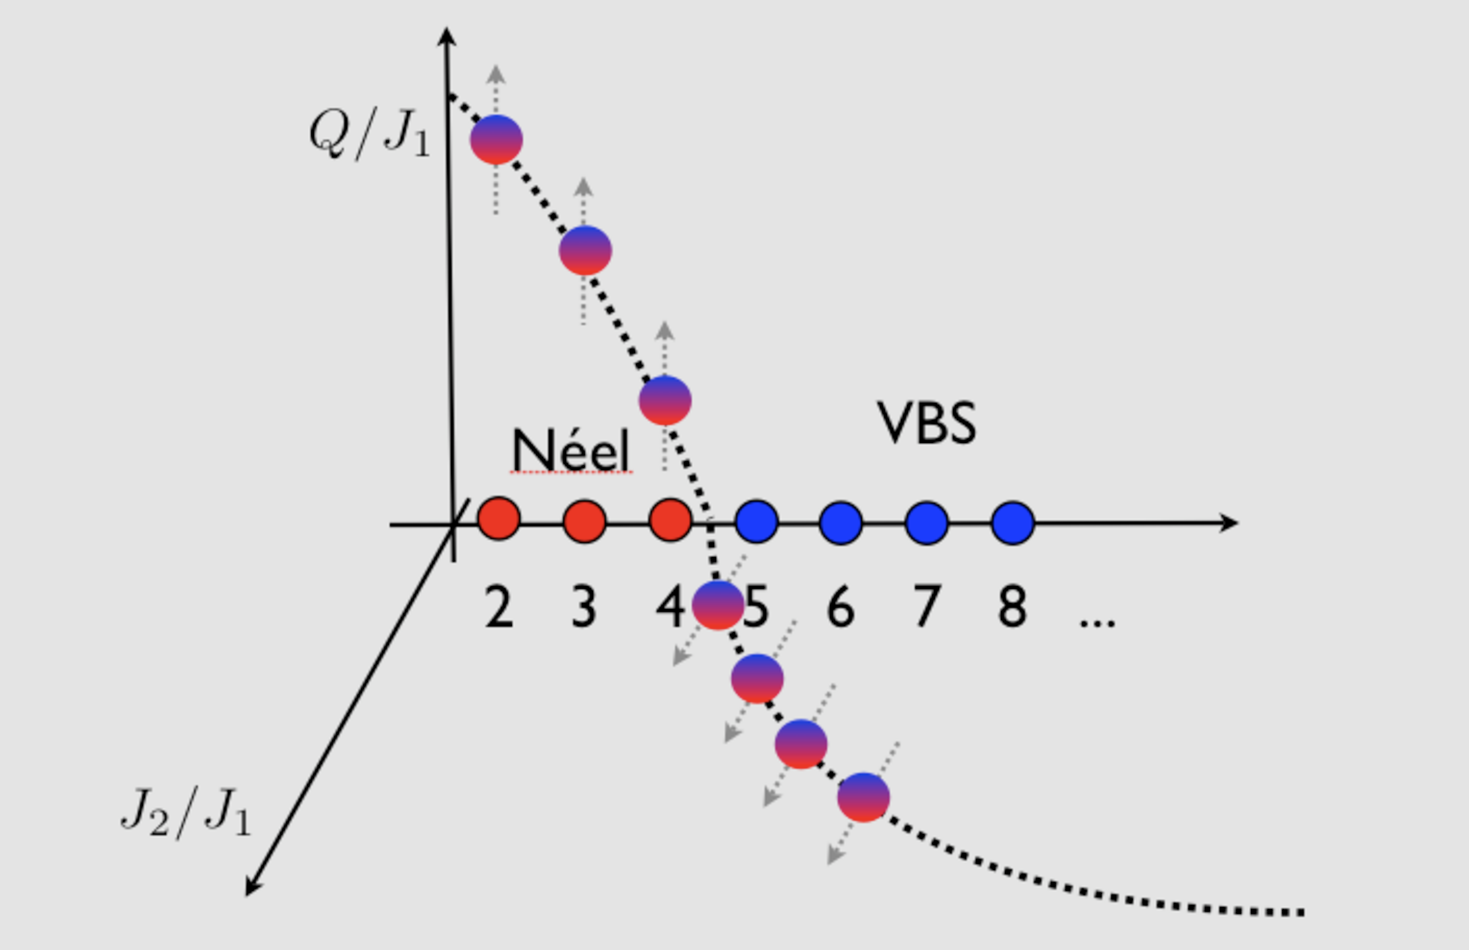
\includegraphics[width=3.5in]{pdj1j2q.pdf}
  \caption{ \label{fig:pdj1j2q} {\em (Will make a better ``quantiative''
      figure when  I am back in Kentucky! -Ribhu)}. Phase Diagram of the
    SU($N$) symmetric sign-problem free
    $J_1$-$J_2$-$Q$ model as a function of $N$. Each of the couplings has been introduced
    in the text: $J_1$ in Sec.~\ref{ss:j1N}; $Q$ in Sec.~\ref{ss:jqN};
  and $J_2$ in Sec.~\ref{ss:j1j2N}. The generalized antiferromagnet
  allows for a detailed unbiased study of deconfined quantum
  criticality at the N\'eel-VBS transition for each value of $N$. }
\end{figure}


\subsection{SU($N$) $J_1$-$Q$ model for $N\leq 4$}
\label{ss:jqN}
In the previous subsection we saw that in two spatial dimensions the
N\'eel-order found for $N=2,3,4$ gives way to valence bond solid
ordered phases for $N\geq 5$ in the SU($N$) symmetric
anti-ferromagnet, Eq~(\ref{ham:j1}). In order to access the quantum
phase transition at a given value of $N\leq 4$ one needs new
``designer'' couplings that
destroy the N\'eel phase and result in the VBS. The first such term discovered was
the so-called $Q$-interaction which can be written in the following
form for any $N$,
\begin{equation}
H_{Q} = - Q \sum_{ab,\langle ijkl \rangle} \left ( T^a_i\cdot
  T^{*a}_j\right ) \left ( T^b_k\cdot T^{*b}_l \right )
\end{equation}
Since the matrix elements of $T\cdot T^*$ are all positive, such a $Q$
coupling is free of the sign problem of quantum Monte Carlo
simulations. Numerical simulations show that $J_1$-$Q$ has N\'eel-VBS
phase transition for $N=2,3,4$. For $N\geq 5$, the $Q$ term strengthens
the VBS that is already present in the $J_1$ only model, and hence to
study the N\'eel-VBS transition for large-$N$, a new designer
Hamiltonian is needed. Before turning to a discussion of such a model in
Sec.~\ref{ss:j1j2N}, let us briefly summarize the nature of the
N\'eel-VBS transition in the SU(2,3,4) $J_1$-$Q$ models.

{\em (show some data here? we need to decide which plots to show
  depending on the space)--Ribhu}

\subsection{SU($N$) $J_1$-$J_2$ model for $N\geq 5$}
\label{ss:j1j2N}

For $N\geq 5$ the $J_1$ model VBS orders and we have seen that the
addition of the $Q$ interaction only strengthens this tendency. We now
introduce an interaction between sites on the same sub-lattice $J_2$ which favors the N\'eel state,
\begin{equation}
H_{J_2}= -J_2 \sum_{a,\langle\langle ij\rangle\rangle} T^a_i\cdot T^{a}_j
\end{equation}
In order to see that this interaction favors the N\'eel state, we note
that in the $H_{J_2}$ model by itself, the two sublattices are
decoupled. The ground state corresponds to having an independent SU($N$) ferromagnet on
each sublattice. Turning on a small $J_1\ll J_2$ interaction will clearly cause
the sub-lattice degeneracy to be lifted, resulting in the
two independent ferromagnets to lock into a single
anti-ferromagnet state. These arguments are true independent of the
value of $N$. We thus
come to the conclusion that for every $N\geq 5$ the VBS state is
realized when $J_1\gg J_2$ and the N\'eel state is obtained when $J_2
\gg J_1$. Thus there must be at least one quantum phase transition as
the ratio
$J_2/J_1$ is tuned. From numerical simulations on $J_1$-$J_2$ model, we have found
evidence for a direct transition between these two phases with no
indication of an intervening phase. 

An important prediction of the deconfined criticality scenario at the
N\'eel-VBS transition is that both N\'eel and VBS order parameters are
simultaneously quantum critical at the phase transition and that space
and time scale in the same way, {\em i.e.} the dynamic critical exponent $z=1$. This implies
that both correlation functions decay as Lorentz-invariant power laws,
\begin{equation}
\label{eq:expdef}
C_{N,V} ({\bf r},\tau) \sim  \frac{1}{~{(\bf r}^2+c^2\tau^2)^{\frac{(1+\eta_{V,N})}{2}}}.
\end{equation}
 where $C_N$ and $C_V$ are the two point correlation functions of the
 N\'eel and VBS order parameters. The indices $\eta_N$ and $\eta_V$
 are the so-called anomalous dimensions of the N\'eel and VBS order
 parameters. The deconfined quantum criticality scenario predicts that
 the continuum field theoretic universality of the N\'eel-VBS critical
 point is described by the non-compact CP$^{N-1}$ universality. Quantitative
 estimates for the universal indices that characterize this
 universality class are available only in the large-$N$
 limit~\footnote{Numerical simulations of lattice discretizations of
   the field theory have been used to make estimates for $N=2$. See
   XXX.}. The $\frac{1}{N}$ expansions for $\eta_N$ and $\eta_V$ are,
\begin{eqnarray}
\label{eq:oneonN}
\eta_N &=& 1 - \frac{32}{\pi^2N}\nonumber\\
1+\eta_V &=& 2 \delta_1 N
\end{eqnarray}
We note here that as $N\rightarrow\infty$, $\eta_N \rightarrow 1$ and
$\eta_V\rightarrow \infty$. Both results are very unusual since
typically order parameters have very small values of the $\eta$
exponent at the critical point. For reference, in the O($N$) model $\eta\rightarrow
0$ in the $N\rightarrow\infty$ limit and $\eta=0.04$ for the O($N=3$) model.

We now turn back to the study of our lattice designer $J_1$-$J_2$-$Q$
Hamiltonian. By studying the size dependence of correlation functions in Eq.~(\ref{eq:expdef})
 at the location of the critical points shown in Fig.~\ref{fig:pdj1j2q}, we can
 estimate values for $\eta_N$ and $\eta_V$ as a function
 of $N$. Our results for $2\leq N \leq 12$ are summarized in Fig.~\ref{fig:exp}. The
 agreement between the large-$N$ expansion and the values obtained from our
 lattice Hamiltonian for a fixed $N$ is quantitative. The lattice
 Hamiltonian also appears to convincingly reproduce the ``smoking gun'' feature that
 $\eta_N=1$ and $\eta_V=\infty$ in the $N\rightarrow \infty$
 limit. All these features lend strong positive support in favor of
 the deconfined quantum criticality scenario at the N\'eel-VBS
 transition in the SU($N$) models considered here.



\begin{figure}
%\centerline{\psfig{figure=fig_exp.pdf,height=6cm}}
  \caption{ \label{fig:exp} Anomalous dimensions of the N\'eel (left)
    and VBS (right)
  order parameters as a function of $N$. The main panels show $\eta_N$ and $\eta_V$ versus $1/N$. For $N=2,3$ and $4$, the data are 
  for the J-Q model, and the results for $N>4$ are for the $J_1$-$J_2$ model. The analytic results 
  from the $1/N$ expansion of the CP$^{N-1}$ field theory are shown as thick red lines. The left and right insets 
  show $N(1-\eta_N)$ and $(1+\eta_V)/N$, respectively. These quantities must be finite in the  $N\rightarrow \infty$ 
  limit according to the DQC theory and should be given by Eq.~(\ref{eq:oneonN}) (solid straight lines in the insets). 
  The next corrections to the exponents have not been computed analytically yet, but we can estimate them approximately 
  as $1+\eta_V = 0.2492 N + 0.68(4)$, $\eta_N = 1+32/(\pi^2 N)-3.6(5)/N^2$ (shown as dashed lines).}
\end{figure}

\subsection{SU($N$) Bilayer}
\label{ss:bilN}

The bilayer geometry provides a simple way to force a trivial paramagnetic
state into the types of SU($N$) models we have discussed in this
section. Consider a bilayer in which each layer is described by some
combination of the $J_1$-$J_2$-$Q$ interactions. Now consider the
following coupling between the layers,
\begin{equation}
 H_{J_\perp} = -J_\perp \sum_{a,[ij]} T^a_i\cdot T^{*a}_j
\end{equation}
where the sum $[ij]$ is taken between spins vertically below each other
in the bilayer. The $J_\perp$ only model has a featureless non-degenerate ground state
consisting of a product of vertical valence bonds. The introduction of intra-layer couplings like the $J_1$-$J_2$-$Q$ interactions will
make the ground state deviate from a simple product state by
increasing the amount of entanglement, but these couplings
 cannot destabilize the featureless paramagnetic
state as long as they are small compared to $J_\perp$. 

{\em (show some data here? we need to decide which plots to show
  depending on the space)-- Ribhu}

\section{U(1) models}
\label{sec:u1models}

One of the main foci of research into designer Hamiltonians is the search, detection and characterization of quantum spin liquid (QSL) phases.  
That is, although there has been much progress in understanding properties of QSL states from effective field theories, there are very few microscopic models amenable to study by QMC that can be argued to exhibit a QSL without controversy.
There have been several high-profile numerical studies that have identified QSL candidates in the last few years, including the apparent resolution of the long-standing question of the kagome-lattice antiferromagnet's QSL groundstate (through large-scale DMRG calculations), and QMC simulations which claim a QSL phase in the half-filled Hubbard model on the honeycomb lattice.  This latter case, which has subsequently become the subject of intense theoretical study, highlights that the synergy between analytical theory and numerics is often driven by the latter.

\subsection{BFG\cite{BFG} Hamiltonians with Z2 spin liquid phases}

Much of the reason for the lack of microscopic models is that fundamental ingredients required to give rise to QSL phases, namely geometrical frustration, are also typical harbingers of the sign problem.  Despite this,  the absence of the sign problem does not fundamentally preclude the existence of spin liquid physics.  In recent years, there has been significant progress in positively identifying (and characterizing) spin liquid phases with QMC.  The most progress has occurred with Hamiltonians with U(1) symmetry -- anisotropic spin or Bose-Hubbard models specifically designed to capture the essential ingredients needed to promote a QSL phase without causing the sign-problem.

%As with many quantum systems, specific Hamiltonians are often difficult to connect directly to experiment.  In the cases where microscopic Hamiltonians are known, they are rarely soluble; hence attempts to reconcile theory and experiment rely on phenomenological low-energy effective theories.  Here again, we see the use of designer Hamiltonians; rather than attempt to solve a potentially complicated approximation to an experimental Hamiltonian, one may instead construct a sign-problem free model which hopefully captures the essential ingredients (e.g. geometric frustration or quantum disorder) which may lead to the desired spin-liquid behavior.

One successful recipe for designing Bose-Hubbard Hamiltonians with QSL phases was pioneered by Isakov and co-workers,\cite{Isakov1, Isakov2, TopoEE} based partly on our understanding of QSL phases from their relation to {\it quantum dimer models}.  Such models have a strong local constraint, that the number of dimers emerging from a site is fixed, as well as quantum tunnelling that allows the state to fluctuate while keeping the constraint satisfied.  Dimer Hamiltonians can be constructed where groundstate superposition of dimer configurations breaks no symmetry -- being a type of QSL (or resonating valence bond) phase.  The features that emerge in this phase can be directly related to special field theories with gauge symmetry and topological order.


\begin{figure}
%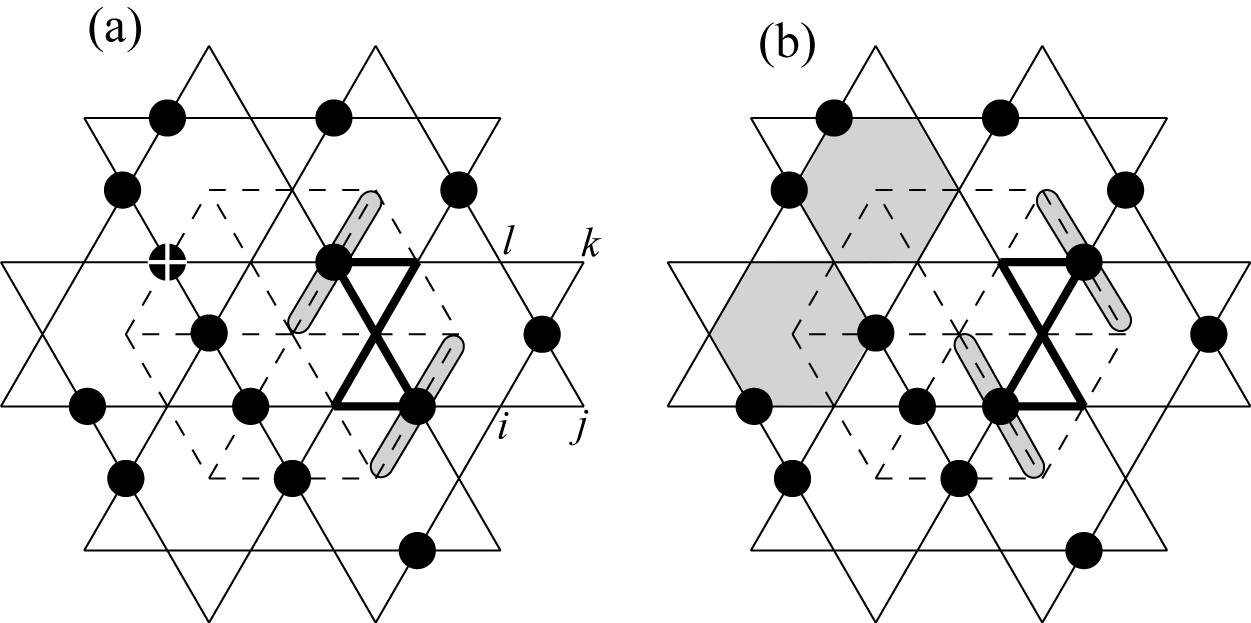
\includegraphics[width=3in]{kagome.pdf}
  \caption{ (a) Boson density in a groundstate configuration satisfying $H_0$ on the kagome lattice.  The degenerate manifold of such configurations maps onto a triangular-lattice (dashed) classical three-dimer configuration, where each boson corresponds to a dimer on the dual lattice.  (b) At right, a plaquette-flip $H_{\rm ring}$ operation preserves the cluster-charging constraint, and can be seen to correspond to a rhombus-flip of dimers.  At left, a charge defect is created by removing one boson (marked ``+'' in (a)).  This defect can be thought of as associating with two hexagonal plaquettes (grey in (b)), each with half of the charge (or two bosons per hexagon), corresponding to fractionalized spinons.}
\end{figure}

The recipe to construct QSL phases in boson models is to map the dimer constraint to a plaquette spin configuration on the dual lattice; the dimer may represents a boson density $n$ configuration on a bond which is frustrated (or unsatisfied).  Then, the role of the quantum dimer tunnelling moves is done by quantum hopping -- processes which are often higher-order in $t$.  Such models are called
{\it cluster-charging} models,\cite{Isakov2} because spin or boson configurations summed over a local cluster (e.g.~a lattice plaquette) are penalized when differing from some chosen value.  For example:
\begin{eqnarray}
%H &=& -t \sum_{\langle ij \rangle} [b^{\dagger}_i b_j + b_i b^{\dagger}_j] + V \sum_{\hexagon} (n_{\hexagon})^2 \\
%H_0 &=& -t \sum_{( ij )} [b^{\dagger}_i b_j + b_i b^{\dagger}_j] + V \sum_{\hexagon} (n_{\hexagon})^2 
H_0 &=& V \sum_{\hexagon} (n_{\hexagon})^2 
\end{eqnarray}
is a cluster-charging potential term which favors three bosons per hexagonal plaquette.  This Hamiltonian alone will promote a highly degenerate manifold of groundstate configurations, where each lattice hexagon satisfies the plaquette constraint but is otherwise disordered.  
Like all Hamiltonian operators which are entirely diagonal in the QMC basis, $H_0$ does not affect the simulation with a sign problem, no matter how the interaction is frustrated.

In order to promote a QSL phase from this classical degenerate manifold, one desires to add quantum fluctuations to this Hamiltonian such that the cluster-charging constraint is not violated.  In this case, a {\it ring-exchange} term, 
\begin{eqnarray}
H_{\rm ring} = -K \sum_{\bowtie} ( b_i^{\dagger} b_j^{\phantom\dagger} b_k^{\dagger} b_l^{\phantom\dagger} + {\rm h.c.} )
\end{eqnarray} 
preserves the cluster-charging constraint $H_0$ while promoting quantum fluctuations.  This, one expects the kagome lattice model with $H = H_0 + H_{\rm ring}$ to retain a disordered groundstate with quantum fluctuations - a good candidate for a quantum spin liquid phase.  In addition, with $K>0$, such terms do not have the sign problem for QMC.

Balents, Fisher and Girvin\cite{BFG} (BFG) were the first to show that variations of this model support the simplest type of Z2 spin liquid -- mainly through exact calculation at a Roksar-Kivelson point in an extended model.\cite{BFG}  Subsequently, using QMC simuations, Isakov and co-workers showed that a variant of the cluster-charging Hamiltonian with short-range hopping 
\begin{eqnarray}
H_{1,3} &=& -t_{1,3} \sum_{( ij )_{1,3}} [b^{\dagger}_i b_j + b_i b^{\dagger}_j]  \\
%H_0 &=& -t \sum_{( ij )} [b^{\dagger}_i b_j + b_i b^{\dagger}_j] + V \sum_{\hexagon} (n_{\hexagon})^2 
%H_0 &=& V \sum_{\hexagon} (n_{\hexagon})^2 
\end{eqnarray}
supports a Z2 spin liquid phase.  Here, the hopping $t$ term can either connect the first, second and third neighbors $( ij )_3$; or it can be nearest-neighbor only $( ij )_1$.  Again, for $t>0$ no sign problem exists.

%Because of the absence of the sign problem and the high probability of promoting a Z2 spin liquid phase based on analytical work, several combinations of the above Hamiltonian terms have now been studied with large scale QMC and demonstrated to have a Z2 spin liquid phase:
%including $H = H_0 + H_3$, $H = H_0 + H_1$, and also $H = H_1 + H_{\rm ring}$, where in the latter case the cluster-charging term is not explicitly required and the Hamiltonian consists of two competing kinetic-energy terms, sometimes called the J-K model.

%The cluster-charging potential term is given by the interaction $V$, which favors 3 bosons per site.  Quantum fluctuations are proportional to $t$: they can be nearest-neighbor\cite{TopoEE} or have equal first, second and third nearest-neighbors\cite{Isakov1,Isakov2}.  This model maps to the three-dimer model on the dual lattice...

%These examples are part of a broader class, originally identified to harbour the simplest Z(2) spin liquid phase at an exactly soluble RK-point, was introduced by Balents, Fisher and Girvin.\cite{BFG}  

The common feature with the BFG Hamiltonians studied by QMC to date is a superfluid to Z(2) spin liquid transition (see Table~XXX).  In the next section, we explore the procedure by which QMC simulations can positively identify such spin liquid phases.  In section \ref{XYstar}, we examine the superfluid to QSL phase transition as an different example of a ``deconfined'' quantum critical point.

\begin{center}
\begin{tabular}{ l | c | c}
  Hamiltonian & Critical Point & References \\
  \hline
  $H_0 + H_1$ & $V/t_1 = 7$ & [\cite{TopoEE}] \\
  $H_0 + H_3$  & $ V/t_3 = 20$? & [\cite{Isakov1,Isakov2}] \\
  $H_1 + H_{\rm ring}$ & $K/t = 22$ & [\cite{Long}]  \\
\end{tabular}
\end{center}

\subsection{Identifying the Z2 spin liquid: Topological Entanglement Entropy}

The smoking gun signature for a spin liquid phase could be argued to be the identification of the emergent gauge symmetry.  It is this symmetry that leads to the concept of topological order in a gapped QSL state.  One manifestation is existence of a ground state degeneracy, which is topological in nature, in the simplest (Z2) case being four-fold on a torus.  Unfortunately, previous QMC studies of QSL states have demonstrated the difficulty in clearly identifying this degeneracy, due to the tendency for tunnelling between the equal-energy states on finite-size lattices with realistic Hamiltonians.  Similarly, recent DMRG work purporting to identify candidate gapped spin liquid states have been unable to identify the associated topological degeneracy.

Luckily, the community has another tool suited for the positive identification of this topological order, through measurements of the entanglement entropy.  Specifically, the scaling of entanglement entropy is predicted to be
\begin{equation}
S_n = a \ell - \gamma + \cdots \label{areaL}
\end{equation}
where subsequent terms scale away at least as fast as $\mathcal{O} (1/\ell)$.  Then, the subleading term to the non-universal ``area law'' ($a \ell$) is a universal correction called the {\it topological entanglement entropy}.  In a gapped QSL phase, it is related to the emergent gauge symmetry (independent\cite{Flammia} of Renyi index $n$), e.g.~in the Z2 spin liquid state $\gamma = 2 \ln(2)$ at $T=0$.

Using the estimators described in Section~\ref{ss:renyi}, it is possible to isolate the topological entanglement entropy from the leading-order area-law, as well as subleading corrections due to corner etceteras, by taking measurements several different geometries A and performing additions or subtractions which isolate only $\gamma$.  For example, the {\it Levin-Wen} regions (illustrated in Fig.~XXX) isolate $2\gamma$ from Eq.~(\ref{areaL}).  For a BFG Hamiltonian discussed in the last section, it is possible to extract the topological entanglement entropy in a QMC simulation.  As discussed by Castelnovo and Chamon through direct calculation on the toric code (which realizes a Z2 fractionalized spin liquid groundstate), the value of $2\gamma$ is approached through two temperature crossovers on a finite-size system, related to the energy of the quasiparticle excitations in the groundstate -- one ``electric'' corresponding to the fractional charge; one ``magnetic'' corresponding to the vison.  Each excitation contributes a value of $\ln(2)$ to the topological entanglement entropy (giving $2\ln(2)$ as $T \rightarrow 0$).  Interestingly, the analogy of the Z2 fractional phase in the kagome BFG Hamiltonian also raises the possibility that, with a suitable ``binding'' potential, an extension of the model with an emergent fermionic excitation might be created.  The demonstration of the existence of a fermionic excitation in a microscopic model without the sign problem would be a major success for simulations of designer Hamiltonians

\subsection{Deconfinement at the XY* transition} \label{XYstar}



%\begin{enumerate}
%\item We have 4 or 5 Hamiltonians (with Z2 \cite{Isakov1} and U(1) spin liquids)
%\item Balents Fisher Girvin gave us a ``recipe'' for creating Hamiltonians with Z2 spin liquids using constrained interactions
%\item The connection to field theory is the emergent gauge structure I guess
%\item Entanglement entropy identifies the emergent gauge structure of the underlying theory
%\item XY*
%\end{enumerate}

\section{Discussion}
\label{sec:discussion}

- Many things left to do along these lines (give some examples), e.g., larger sizes are still needed
to fully characterize N\'eel--VBS transition; parallelization of QMC, impurities, disorder

- Fermions: it should be possible to study 1 or 2 fermions (manageble sign problem) in 
VBS/critical/spin-liquid systems. One should be able to see some aspects of the "strange metal''.
Mention meron algorithm---perhaps some more interesting designer hamiltonian can be constructed.

- Open fundamental questions in this approach, e.g., can one design a sign-problem-free
  SU(2) hamiltonian with a spin liquid phase?

- Non-equilibrium QMC


In Ref.~X, Troyer and Wiese presented a proof that the sign problem cannot be solved in general. The problem is here
defined in terms of constructing a QMC algorithm for which the computational effort scales as a power-law in the system
size. They show a particular problem for which the removal of the sign still leaves a problem for which the Monte Carlo
sampling is believed to scale exponentially in the system size. However, the problem chosen is that of a spin glass, and 
the conclusion is that the quantum spin glass is not easier to solve than the corresponding classical spin glass. This is 
hardly a surprising result, and the proof does not say anything about QMC solutions of systems that are not directly
associated with the well known difficulties of simulating classical glassy systems with complicated energy landscapes. 
Whether or not the sign problem can be circumvented for translationally invariant systems such as fermionic Hubbard models 
and frustrated quantum spins models remains and open question.


% Create the reference section using BibTeX:
\bibliography{rev_bib.bib}
\bibliographystyle{Science}
%\bibliographystyle{apsrev}

\end{document}

